%********BEGIN PREAMBULE*********
\documentclass[14pt,a4paper]{report}

\usepackage[14pt]{extsizes}
\usepackage{cmap}
\usepackage[T2A]{fontenc}
\usepackage[utf8]{inputenc}
\usepackage[english,russian]{babel}
\usepackage{pscyr}

\usepackage{graphicx}
\usepackage{amssymb,amsfonts,amsmath,amsthm}
\usepackage{lscape}
\usepackage{makecell}
\usepackage{multirow}
\usepackage{ulem}
\usepackage{indentfirst}
\usepackage{setspace}
\usepackage{color}
\usepackage{tabularx}
\usepackage{titlesec}
\usepackage{hyperref}
\hypersetup{pdfborder = 0 0 0}
\usepackage{tocloft}
\usepackage{listings}
\usepackage{float}

% Ключевые слова
\newcommand{\kwTitle}{%%report-title%%}
\newcommand{\kwPlace}{%%report-city%%}
\newcommand{\kwYear}{%%report-year%%}
\newcommand{\kwAuthorName}{%%report-author-name%%}
\newcommand{\kwAuthorFaculty}{%%report-author-facility%%}
\newcommand{\kwAuthorSpeciality}{%%report-author-speciality%%}
\newcommand{\kwAuthorDepartment}{%%report-author-department%%}
\newcommand{\kwAuthorInfo}{%%report-author-info%%}
\newcommand{\kwTeacherName}{%%report-teacher-name%%}
\newcommand{\kwTeacherTitle}{%%report-teacher-title%%}
\newcommand{\kwTeacherInfo}{%%report-teacher-info%%}

\lstset{
	language=C++,                % choose the language of the code
	basicstyle=\footnotesize\ttfamily,       % the size of the fonts that are 
	%used for 
	%the code
	numbers=left,                   % where to put the line-numbers
	numberstyle=\footnotesize,      % the size of the fonts that are used for 
	%the line-numbers
	stepnumber=1,                   % the step between two line-numbers. If it 
	%is 1 each line will be numbered
	numbersep=5pt,                  % how far the line-numbers are from the 
	%code
	backgroundcolor=\color{white},  % choose the background color. You must 
	%add \usepackage{color}
	showspaces=false,               % show spaces adding particular underscores
	showstringspaces=false,         % underline spaces within strings
	showtabs=false,                 % show tabs within strings adding 
	%particular underscores
	%frame=single,           % adds a frame around the code
	tabsize=2,          % sets default tabsize to 2 spaces
	captionpos=b,           % sets the caption-position to bottom
	breaklines=true,        % sets automatic line breaking
	breakatwhitespace=false,    % sets if automatic breaks should only happen 
	%at whitespace
	escapeinside={\%*}{*)},          % if you want to add a comment within 
	%your code
	%keywordstyle=\color{blue},
	%stringstyle=\color{red},
	%commentstyle=\color{green}
}

\usepackage[tableposition=top]{caption}
\usepackage{subcaption}
\DeclareCaptionLabelFormat{gostfigure}{Рисунок #2}
\DeclareCaptionLabelFormat{gosttable}{Таблица #2}
\DeclareCaptionLabelSeparator{gost}{~---~}
\captionsetup{labelsep=gost}
\captionsetup[figure]{labelformat=gostfigure}
\captionsetup[table]{labelformat=gosttable}
\renewcommand{\thefigure}{\arabic{figure}}
\renewcommand{\thesubfigure}{\asbuk{subfigure}}

\onehalfspacing % полуторный интервал
\renewcommand{\rmdefault}{ftm} % Times New Roman
\frenchspacing % не всталять дополнительный пробел в конце предложения
%\spaceskip .45em plus .4em minus .0em

\usepackage{geometry} % поля
\geometry{left=3cm}
\geometry{right=1cm}
\geometry{top=2cm}
\geometry{bottom=2cm}

\usepackage{fancyhdr} % колонитулы
\pagestyle{fancy}
\fancyhf{}
\fancyhead[L]{\it\color[gray]{0.9}\kwTitle}
\fancyfoot[R]{\thepage}
\fancyheadoffset{0mm}
\fancyfootoffset{0mm}
%\setlength{\headheight}{17pt}
%\setlength{\footheight}{17pt}
\renewcommand{\headrulewidth}{0pt}
\renewcommand{\footrulewidth}{0pt}
\fancypagestyle{plain}
{
    \fancyhf{}
    \fancyhead[L]{\it\color[gray]{0.8}\kwTitle}
    \fancyfoot[R]{\thepage}
}

% Заголовки

\titleformat{\chapter}
    {\bfseries}
    {\thechapter.}
    {1em}{}
 
\titleformat{\section}
    {\normalsize\bfseries}
    {\thesection}
    {1em}{}
 
\titleformat{\subsection}
    {\normalsize\bfseries}
    {\thesubsection}
    {1em}{}

% Оглавление

\newcommand{\prechapterheading}[1]{
	\clearpage 
    \begin{center}
    \textbf{#1}
    \end{center}
}

\makeatletter
\newif\if@prechapterused
\@prechapterusedfalse

\newcommand{\l@prechapter}[2]{#1\cftdotfill{\cftdotsep}#2\par}
\newcommand{\prechapter}[1]{
	%\chapter{#1}    
    \prechapterheading{#1}
    \@prechapterusedtrue
    \addcontentsline{toc}{chapter}{#1}
}

\let\oldchapter\chapter

\renewcommand{\chapter}[1]
{
\if@prechapterused\vspace{-2em}\@prechapterusedfalse\fi
\begingroup
	\let\clearpage\relax
	\let\cleardoublepage\relax
	\oldchapter{#1}
\endgroup
}
\makeatother

\renewcommand{\cfttoctitlefont}{\hspace{0.38\textwidth} \bfseries}
\renewcommand{\cftbeforetoctitleskip}{-1em}
\renewcommand{\cftaftertoctitle}{\mbox{}\hfill \\ \mbox{}\hfill{\footnotesize Стр.}\vspace{-2.5em}}
\renewcommand{\cftchapfont}{\normalfont}
\renewcommand{\cftchapdotsep}{\cftdotsep}
\renewcommand{\cftchapleader}{\normalfont\cftdotfill{\cftchapdotsep}}
\renewcommand{\cftchappagefont}{\normalfont}
\renewcommand{\cftsecfont}{\hspace{31pt}}
\renewcommand{\cftsubsecfont}{\hspace{11pt}}
\renewcommand{\cftbeforechapskip}{1em}
\renewcommand{\cftbeforesecskip}{1em}
\renewcommand{\cftsecindent}{-0.5em}
\renewcommand{\cftparskip}{-2mm}
\renewcommand{\cftdotsep}{1}
\setcounter{tocdepth}{1} % задать глубину оглавления — до section включительно

% Настройка вертикальных и горизонтальных отступов в заголовках
\titlespacing*{\chapter}{\parindent}{*4}{*0}
\titlespacing*{\section}{\parindent}{*4}{*4}
\titlespacing*{\subsection}{\parindent}{*0}{*0}

\setlength{\parindent}{15mm} % абзацный отступ

\newcommand{\handtextplace}[2][50px]
{
	\parbox{#1}{
	\begin{center}
		{~}\\[-0.005\textheight]
		\underline{\hspace{#1}}
		\\[-0.005\textheight]\footnotesize{#2}
	\end{center}
	}
}

\newcommand{\textplace}[2]
{
	\parbox{\textwidth}{
	\begin{center}
		{~}\\[-0.005\textheight]
		#1
		\\[-0.005\textheight]\footnotesize{(#2)}
	\end{center}
	}
}

\begin{document}

\thispagestyle{empty}

\begin{small}

\begin{center}
\textbf{Министерство образования и науки Российской Федерации}\\
Федеральное государственное бюджетное образовательное учреждение высшего профессионального образования\\
\textbf{<<НАЦИОНАЛЬНЫЙ ИССЛЕДОВАТЕЛЬСКИЙ\\ТОМСКИЙ ПОЛИТЕХНИЧЕСКИЙ 
УНИВЕРСИТЕТ>>}\\
\end{center}
\hrule

\begin{flushleft}
Институт \hspace{2em} \kwAuthorFaculty\\
Направление подготовки (специальность) \hspace{2em} \kwAuthorSpeciality\\
Кафедра \hspace{2em} \kwAuthorDepartment\\
\end{flushleft}

\vspace{5pt}

\begin{center}
\textbf{ПОЯСНИТЕЛЬНАЯ ЗАПИСКА}\\
\textbf{к творческому проекту}\\
\end{center}
по дисциплине <<\kwTitle>>

\noindent\begin{tabularx}{\textwidth}{Xrr}
\raggedright{Выполнил} \kwAuthorInfo & \handtextplace[100pt]{(подпись)} & 
\kwAuthorName\\*[-30pt]
~ & ~ &
\handtextplace[30pt]{~}~\handtextplace[100pt]{(дата 
сдачи)}~20\handtextplace[20pt]{~}г.\\*[10pt]
\kwTeacherTitle & \kwTeacherInfo & 
\kwTeacherName\\*[0pt]
~ & \handtextplace[100pt]{(оценка руководителя)} & 
\handtextplace[100pt]{(подпись)}\\*[-20pt]
~ & ~ & 
\handtextplace[30pt]{~}~\handtextplace[100pt]{(дата 
проверки)}~20\handtextplace[20pt]{~}г.\\*[10pt]
Творческий проект & студент \kwAuthorName & выполнил и защитил\\*[0pt]
~ & ~ & с оценкой \handtextplace[100pt]{~}\\*[-30pt]
Члены комиссии: & \handtextplace[100pt]{~} & ~\\*[-30pt]
~ & \handtextplace[100pt]{~} & ~\\*[-30pt]
~ & \handtextplace[100pt]{~} & ~\\*[-30pt]
~ & ~ & 
\handtextplace[30pt]{~}~\handtextplace[100pt]{(дата 
защиты)}~20\handtextplace[20pt]{~}г.\\*[10pt]
\end{tabularx}

\vspace{30mm}

\noindent{
\kwPlace~\kwYear~г.
}

\end{small}

\newpage

\vspace*{-3em}

\chapter{Задание}
В рамках проектной деятельности студенту необходимо создать программное 
обеспечение для отображения единого расписания для студентов элитного 
технического образования. Данный продукт должен объединять расписание 
основного потока и элитного с учетом дублирующихся в основном и элитном потоке 
предметов, а также предупреждать о пересечениях между предметами. В конце 
своей работы студент должен получить сайт, который будет генерировать 
расписание для каждого студента ЭТО, с учетом его групп (основной и элитной).

\chapter{Реферат}
\begin{enumerate}
\item Программирование демо-версии сайта

\item Отладка сайта

\item Поиск недостатков

\item Исправление недостатков

\item Тестирование сайта

\item Реклама сайта среди студентов-элитников
\end{enumerate}
\newpage

\tableofcontents
\newpage

\vspace*{-12pt}
\chapter{Определения}

\textbf{HTML5 (HyperText Markup Language, version 5)} --- язык для 
структурирования и 
представления содержимого всемирной паутины.

\textbf{CSS3 (Cascading Style Sheets 3)} --- формальный язык разметки, 
используемый как 
средство описания и оформления внешнего вида веб-страниц

\textbf{JavaScript} --- прототипно-ориентированный сценарный язык 
программирования, 
встраиваемый в браузер для программного доступа к объектам приложений

\textbf{AJAX (Asynchronous Javascript and XML)} ---  подход к построению 
интерактивных 
пользовательских интерфейсов веб-приложений, заключающийся в «фоновом» обмене 
данными браузера с веб-сервером. В результате, при обновлении данных 
веб-страница не перезагружается полностью, и веб-приложения становятся быстрее 
и удобнее.

\textbf{PHP} --- скриптовый язык программирования общего назначения, 
интенсивно 
применяемый для разработки веб-приложений

\chapter{Обозначения и сокращения}

\textbf{ЭТО} - Элитное Техническое образование

\chapter{Введение}

	Как известно всем студентам Национального Исследовательского Томского  
Политехнического Университета, обучающимся по программе Элитного технического 
образования, есть расписание групп основного потока и потока 
ЭТО. Проблема заключается в том, что расписание для групп потока ЭТО не 
соединено с расписанием основного потока из-за чего возникает множество 
неудобств: приходится выписывать/вычерчивать себе отдельное расписание, 
которое неизбежно меняется, в конечном счете, этот листочек с расписанием 
теряется и все начинается сначала. Тем, кто пытается просто запомнить свое 
расписание еще труднее: приходится запоминать 4 недели, так как есть нечетная 
+ четная для основного потока и нечетная + четная для  группы ЭТО. 

\newpage
\chapter{Цели и задачи проекта}

\begin{itemize}
\item Разработка концепции проекта, рабочего плана и плана развития проекта
\item Определение потребностей студентов элитного технического образования
\item Программирование beta-версии сайта, с учетом привычного дизайна для 
студентов ТПУ
\item Внешнее тестирование среди целевой аудитории, а именно студентов 
элитного технического образования
\end{itemize}

\chapter{Результаты выполнения проекта}

В ходе проделанной работы был разработан законченный программный продукт в 
виде Web-приложения для студентов элитного технического образования. Данный 
продукт был выполнен с помощью соверменных средств разработки Web-приложений, 
таких как HTML5, CSS3, AJAX, JavaScript, PHP. В ходе beta-тестирования, 
проведенного 
среди целевой аудитории, было выявлено, что данный сервис быстрый и удобный 
для конечного пользователя и позволяет экономить ценное для студентов время, 
которое он может потратить на учебу, вместо того, чтобы вручную решать 
проблему с расписанием.

\chapter{Список использованных источников}

\begin{enumerate}
  \item http://php.net/docs.php --- Документация по языку программирования PHP
  \item http://htmlbook.ru/ --- Документация по HTML5
  \item http://es5.javascript.ru/ --- Документация по языку программирования 
  JavaScript
  \item http://javascript.ru/ajax --- Учебник по AJAX и COMET
\end{enumerate}

\chapter{Перечень использованных программных продуктов}

\begin{enumerate}
  \item \textbf{SublimeText} --- быстрый кроссплатформенный редактор исходных 
  текстов программ.
  \item \textbf{Apache} --- свободный веб-сервер.
\end{enumerate}

\newpage
\chapter{Приложения}

\begin{figure}[H]
\centerline{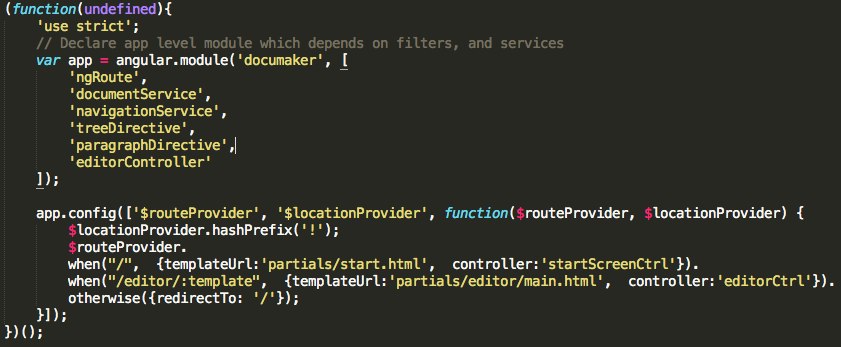
\includegraphics[scale=0.8]{gfx/1.png}}
\caption{Главня страница приложения}
\label{fig1}
\end{figure}

\begin{figure}[H]
\centerline{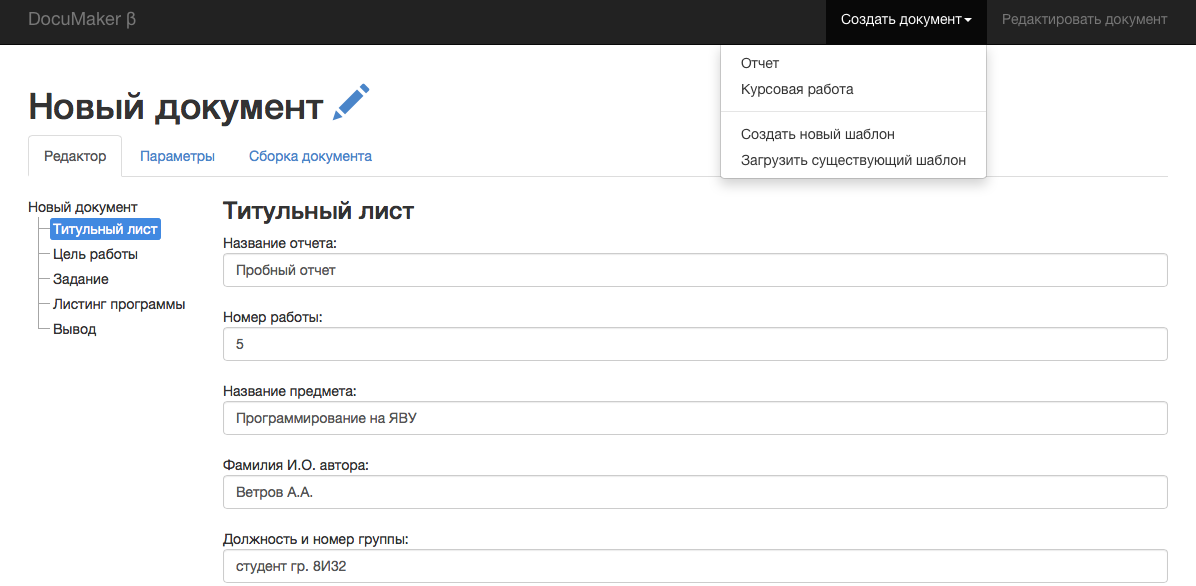
\includegraphics[scale=0.75]{gfx/2.png}}
\caption{Пример работы приложения}
\label{fig2}
\end{figure}

\begin{figure}[H]
\centerline{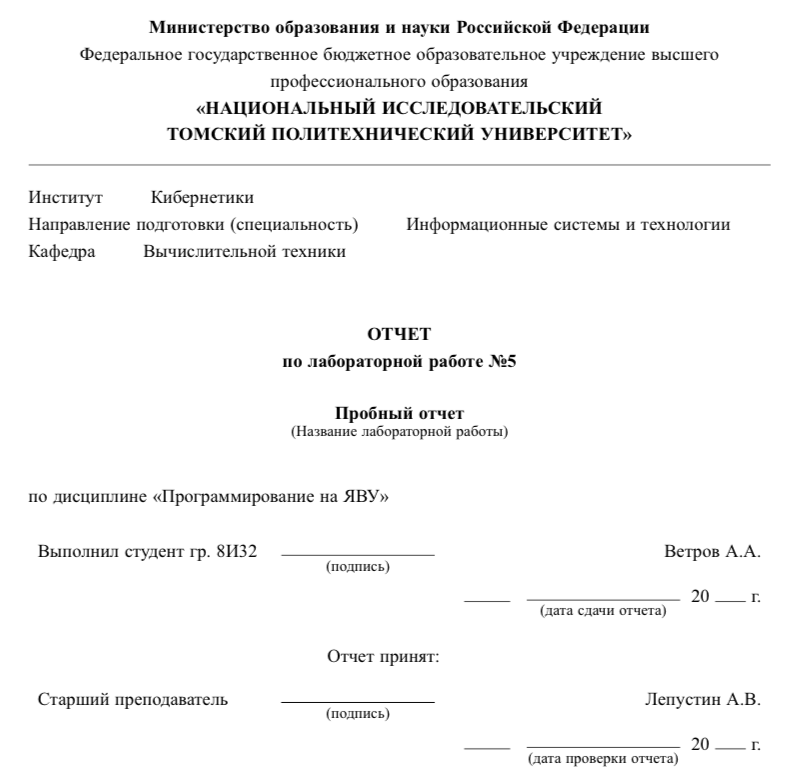
\includegraphics[scale=0.55]{gfx/3.png}}
\caption{Диаграмма Ганта}
\label{fig3}
\end{figure}

\end{document}